


\begin{figure}[H]
  \centering
  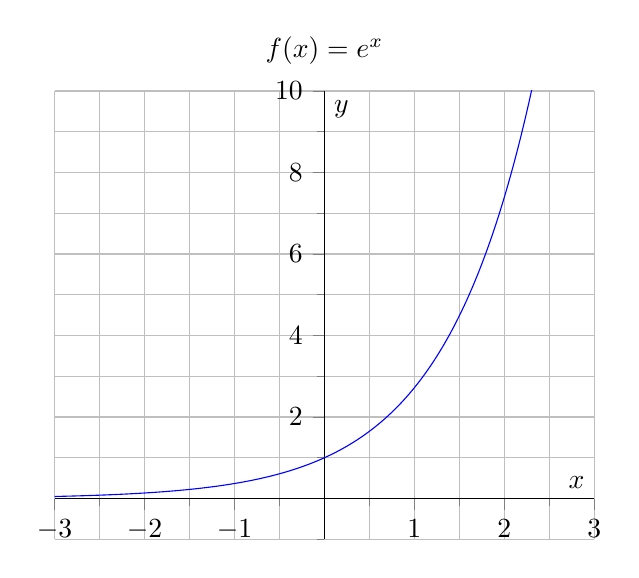
\begin{tikzpicture}
    \begin{axis}[
      xmin=-3, xmax=3,
      ymin=-1, ymax=10,
      axis x line=middle,
      axis y line=middle,
      axis line style={-},
      tick align=outside,
      grid=both,
      minor tick num=1,
      xlabel={$x$},
      ylabel={$y$},
      title={$f(x)=e^x$}
    ]
      \addplot[blue, domain=-3:3, samples=200] {exp(x)};
    \end{axis}
  \end{tikzpicture}
  \caption{Função exponencial $f(x)=e^x$.}
\end{figure}